% !TEX root = proposal.tex

\section{Methodology (Proposed Algorithms)}
This section outlines the steps and algorithms proposed for the audio signal processing project, focusing on feature extraction, similarity metrics, and applications.

\subsection{Feature Extraction}
At a high level, we aim to accomplish the following hierarchical feature extraction:
\begin{quote}
\begin{fixmathspace}
\begin{flalign*}
    \text{raw audio} &\rightarrow \text{frequencies/tones (e.g. via FFT)}&&\\
    &\rightarrow \text{fundamentals/notes}&&\\
%    &\rightarrow \text{key, reference pitch (TBD)}&&\\
    &\rightarrow \text{functional harmony/chords and sequences}&&\\
    &\rightarrow \text{topics/genres (e.g. via LDA)}
\end{flalign*}
\end{fixmathspace}
\end{quote}

\begin{enumerate}
    \item In order to extract notes, we analyze harmonic information to identify fundamental tones. We may be able to distinguish them from overtones based on the quirks of equal tempered tuning (see Figure $\ref{fig:12tet_spiral}$ for a visualization of the discrepancy between 12-tet and pure harmonics). We will likely require high resolution on the frequency axis, if we are to distinguish between natural harmonics and tempered tones. If high resolution Short-Time Fourier Transform algorithms are prohibitively slow, perhaps we can use QISP \cite{Smith2011}. See Figure $\ref{fig:qisp}$ for some preliminary test results, rendered in a custom visualization we developed for comparing spectrograms to a musical scale.
    \item From note information, we can infer the key and reference pitch, to provide context for the harmonic information. These may be useful metadata in themselves for other processes, but in this pipeline we expect they will mainly be ``factored out'' so we can focus on functional harmony independently.
    \item Given a collection of notes, we can analyze intervalic relationships to derive harmonic functions and identify chords, which will be the primary terms in our subsequent analysis. A degree of reductionism is inherent in functional analysis; our selection of how to encode chordal information will largely determine the capacity of models to detect similarities and differentiate pieces of music.
    \item Finally, we can analyze all the chords and sequences thereof in a corpus, to perform topic extraction. Such high-level features can be used in subsequent calculation of similarity metrics between pieces of music and similarity-based search functions.
\end{enumerate}

\begin{figure}[H]
    \centering
    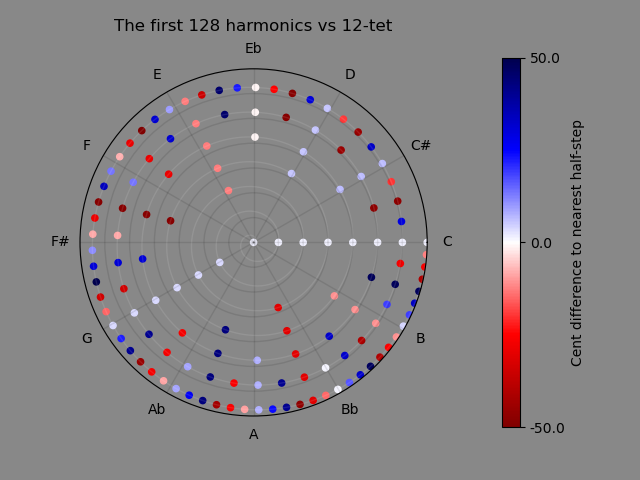
\includegraphics[scale=0.67]{12tet_spiral.png}
    \caption{An illustration of the relationship between equal tempered tuning and natural harmonics}
    \label{fig:12tet_spiral}
\end{figure}

\begin{figure}[H]
    \centering
    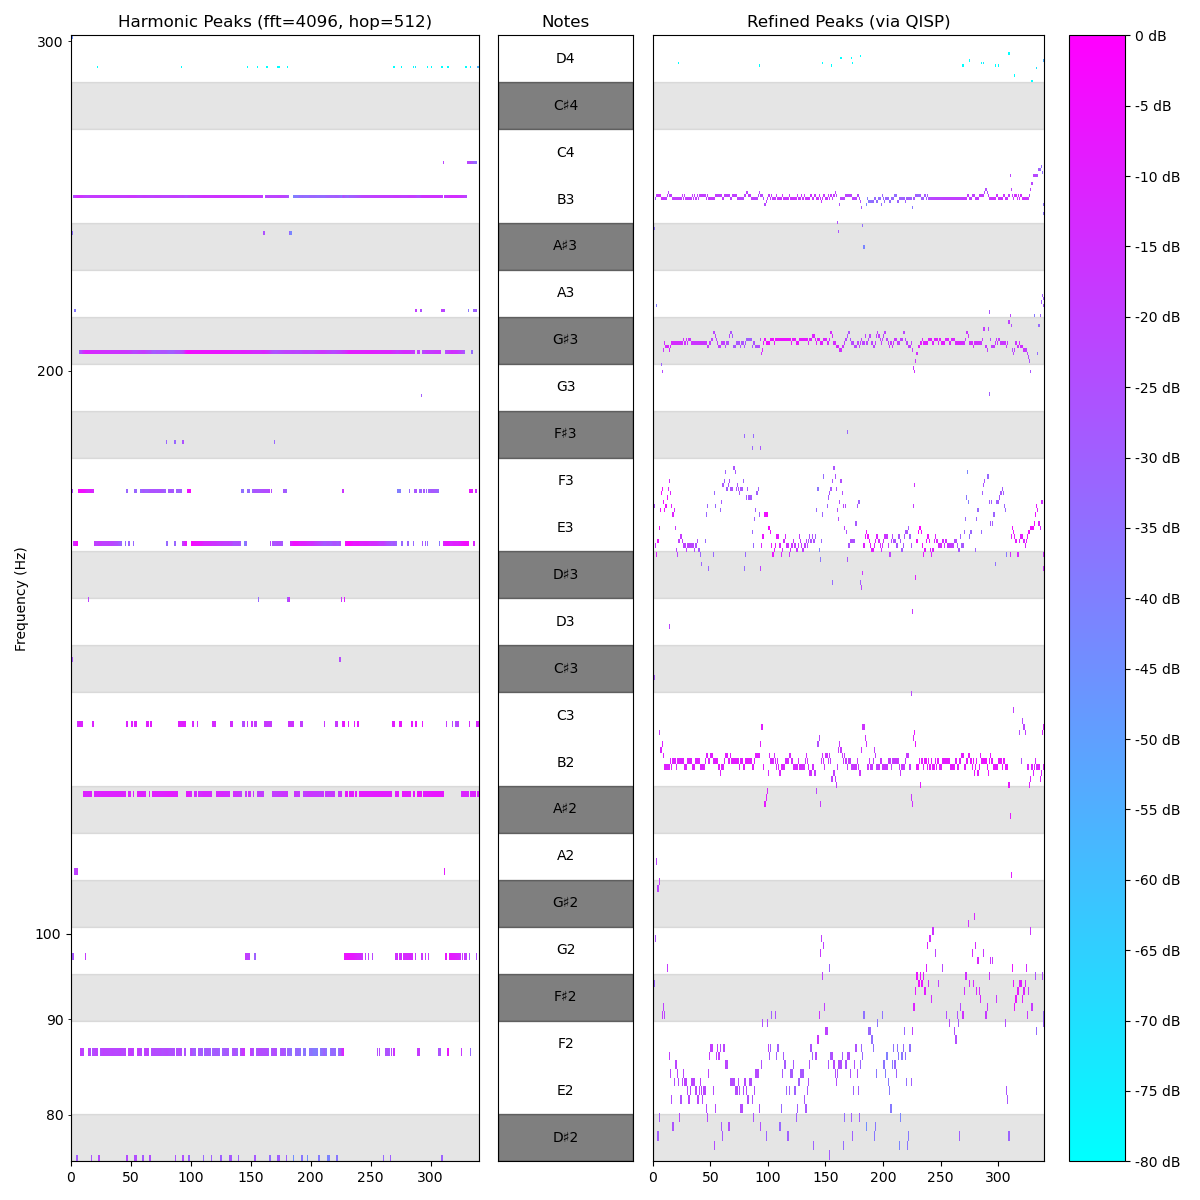
\includegraphics[scale=0.40]{qisp.png}
    \caption{Lower notes (e.g. B2) are particularly susceptible to quantization error}
    \label{fig:qisp}
\end{figure}

\newpage
\subsection{Similarity Metrics}
To compare different pieces of music and identify similarities, we will employ various metrics such as Cosine Similarity, TFIDF, and market basket analysis metrics (e.g. Jaccard Index).

\subsection{Applications}
The extracted features and similarity metrics can be utilized in several applications:
\begin{itemize}
    \item Audio playback and visualization of extracted features.
    \item Implementation of a search by similarity/dissimilarity feature.
    \item Automated playlist creation based on the similarity of songs.
\end{itemize}

\subsection{Challenges}
The primary challenge anticipated is the ambiguity prevalent in various stages, from fundamental detection to chord assignment. This work will focus on functional harmony in the context of a twelve-tone equal-tempered tuning system, aiming for extensibility to a broader analytical framework in future developments.
